\documentclass[10pt,journal,compsoc,draftclsnofoot]{IEEEtran}

% Definition of \subparagraph
\makeatletter
\newcommand\subparagraph{%
  \@startsection{subparagraph}{5}
  {\parindent}
  {3.25ex \@plus 1ex \@minus .2ex}
  {0.75ex plus 0.1ex}
  {\normalfont\normalsize\bfseries}}
\makeatother

\newcounter{subparagraph}[paragraph]

\usepackage{listings}
\usepackage{titlesec}
\usepackage{float}
\usepackage{hyperref}
\usepackage{array}
\usepackage{tocloft}
\usepackage{lscape}
\usepackage{textcomp}
\usepackage{pgfgantt}
\usepackage{amsmath}

\usepackage{geometry}
\geometry{margin=0.75in}

\setcounter{tocdepth}{4}
\setcounter{secnumdepth}{4}

\begin{document}
\onecolumn

\begin{titlepage}
\null
\vspace{15mm}

\begin{flushleft}
\begin{bfseries}
	\vskip2mm
	\Huge{Midterm Progress Report for\\ Better Graphics For A Robotics Grasping GUI}\\
	\vspace{15mm}
	\textbf{\huge Shady Robots} \\
	\vskip2mm
	\large{Group 12}
	\vskip5mm
	\Large{Justin Bibler \\
	Matthew Huang \\
	Daniel Goh \\}
\end{bfseries}

\vspace{15mm}
\Large{CS462: Senior Software Engineering Project} \\
\Large{Winter 2017} \\

\vspace{5mm}

\today

\vfill

\begin{normalsize}
{\bf Abstract:}
This document goes over the project our project's purpose and goal, as well as providing an update on our team's progress with the project.
The retrospective section details the positives, deltas, and actions of each week, which will be used from here on out to allow the team to reflect and improve for the remainder of the project timeline.

{\bf Keywords:} OpenInventor, OpenGL, OpenRAVE, shaders, warm cool shaders, silhouettes, shadows, robotic simulation, geometry, visualization, render, vertex lines, retrospective, positive, delta, action
\end{normalsize}
\end{flushleft}

\newpage

\end{titlepage}

\begin{flushleft}

\section{Project Purpose and Goals}
The purpose of our project is to update the graphics of an existing program that creates a simulation of a robotic arm grasping objects.
The reasoning behind our desire to update the graphics is because our client is using online data collection methods using these visualizations.
However, the outdated graphics are making it difficult for users to give confident responses to the survey.
To fix this problem, we have created 4 major goals:
\begin{enumerate}
\item Implement Gooch shading.
\item Implement shadows.
\item Implement silhouettes.
\item Test to ensure our implementations improve user confidence using interviews.
\end{enumerate}

\section{Where we are in the project}
We created an installation guide to properly install OpenRAVE from source with the qtcoinrave plugin with our changes.
Our system is currently running Ubuntu 14.04 and the GLSL version for the code is GLSL 1.2.
These versions are required to successfully compile and run OpenRAVE from source with our installation guide.
Currently in our project, we have implemented warm cool shaders, and shadows into OpenRAVE.

\begin{figure} [H]
  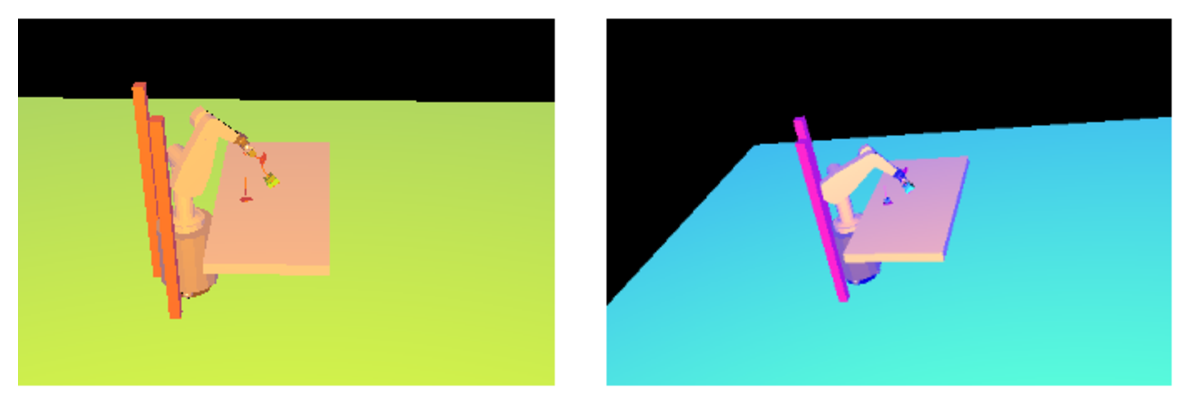
\includegraphics[scale=0.8]{Warmcool.eps}
  \caption
{ \newline \hspace{\linewidth}
Figure showing OpenRAVE simulation with warm cool shaders}
  \label{fig:Warmcool}
\end{figure}

\begin{figure} [H]
  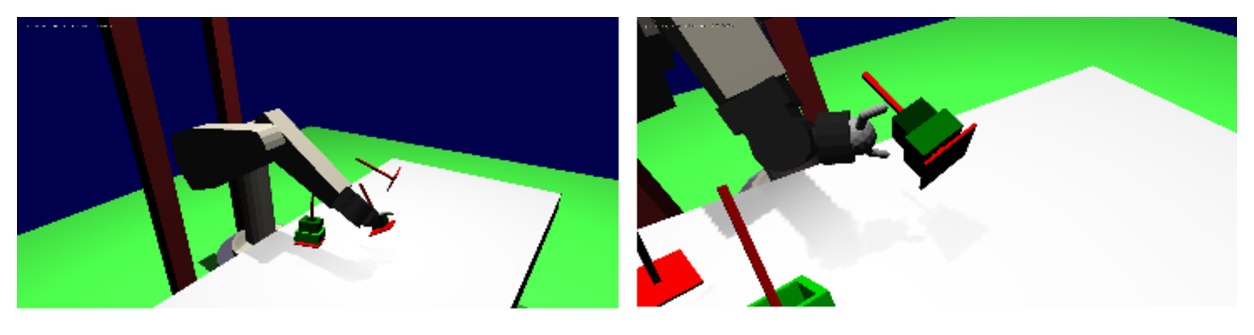
\includegraphics[scale=0.8]{Shadows.eps}
  \caption
{ \newline \hspace{\linewidth}
Figure showing OpenRAVE simulation with shadow shaders}
  \label{fig:Shadow}
\end{figure}

We also have a silhouette shader written out. However, due to the lack of API documentations, we have yet to implement them.

\begin{figure} [H]
  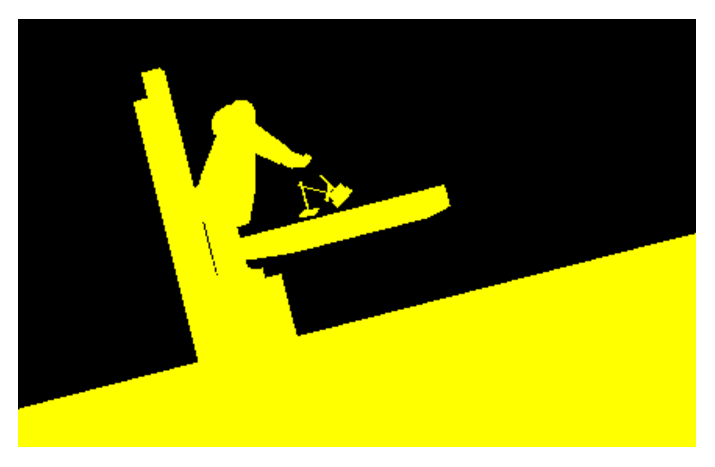
\includegraphics[scale=0.8]{Silhouette.eps}
  \caption
{ \newline \hspace{\linewidth}
Silhouette shader renders and enlarge version of an object that is meant to be drawn in the background (it is drawn in yellow for visibility's sake).}
  \label{fig:Silhouette}
\end{figure}

\section{What is left to do}
We need to implement the silhouette shaders into the qtcoinrave plugin.
Then, we will need to combine the warm cool shaders, shadows, and silhouettes to run simultaneously.
After the implementations are completed, we will maintain and polish the code to ensure optimal performance of the OpenRAVE simulation.
We will then run surveys to determine if our team's implementation have improved the visuals of the OpenRAVE simulation.

\newpage

\section{Problems and Solutions}
\subsection{Justin Bibler}
\textbf{Implementing Shadows and Related Problems}
\par
The first problem I had was figuring out how to implement shadows.
My major difficulty was that qtcoin doesn't automatically render twice, which is a requirement for shadow shading.
However, I was able to find a solution by searching through an extended library for Coin3D that our current source code did not use.
This library contained a built-in shadow class that did double rendering and had built-in shadow shaders.

\vspace{3mm}

The next problem that I came across was determining how to implement the shadow class into the source code.
This was a difficulty because there is minimal documentation on how to use the shadow class.
I was able to overcome this problem by reading the class hierarchy table in the documentation and extensively testing different ways of implementing the shadow class.

\vspace{3mm}

Finally, our current implementation of the shadows overrides all the other shaders.
This makes it so that the warm cool and silhouette shaders cannot be run at the same time.
I am currently working on a solution to fix this.
My current plan is to combine the shadow shaders into our warm cool and silhouette shader implementations, and override the default shadow shaders with these new combined shaders.

\newpage

\subsection{Matthew Huang}
\textbf{Implementing Silhouette Shaders}
\par
The problems that I ran into are similar to the problems that Justin ran into, which is that we have no control over the built-in rendering.
Without control over the render loop, the silhouette shaders cannot be implemented into the simulation because silhouettes require two rendering passes.
Additionally, for the current silhouette shaders, we will need access to the depth mask and the glCullFace function.
These functions will allow us to keep the silhouette in the background and the robotic arm in the foreground.
The silhouettes, at the moment, are simply being enlarged, colored black, and then drawn with the current qtcoin configurations.
If the qtcoin API does not give us access to these functions, we will have to find a work around solution for the silhouettes.
\par
One possible solution that I am currently investigating is using the geometry shader to implement the silhouettes.
The geometry shader lives between the vertex and fragment shaders so it will not affect our warm cool and shadow implementations.
Additionally, geometry shader silhouettes appear to only require a single rendering pass which would solve the qtcoin API issues that our group keeps running into.
Unfortunately, the geometry shader silhouettes are also reliant on how the object is drawn; if it does not have the correct triangle pattern, then it is unlikely to work.
Since I don't know how the scene is being drawn in terms of vertex patterns, this solution is still tentative.

\vspace{3mm}

\textbf{Modifying The Existing Warm Cool Shaders}
\par
As for the warm cool shaders, the code that Julio Medina provided us was a good starting point for our implementation.
He, for the most part, had correct lighting, normal vectors, and eye/model positions.
The only part of his code that I really had to modify was his color computations.
The color computations that he ran over saturated the scene with too much orange.
I replaced his color equation with the glsl mix function which linearly interpolated between the augmented cool and warm colors.
This added a greater range of colors for our scene.
This difference can be seen in the two images in figure 1 below.

\begin{figure} [H]
  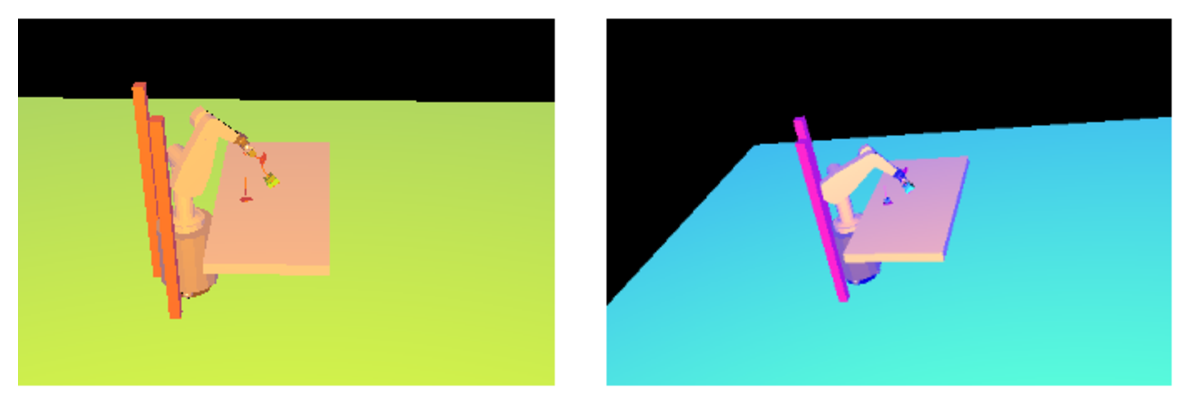
\includegraphics[scale=0.8]{Warmcool.eps}
  \caption
{ \newline \hspace{\linewidth}
Figure showing how my implementation creates a greater range of colors in the OpenRAVE scene}
  \label{fig:Warmcool}
\end{figure}

Now, all that is left to do with the warm cool shading is to implement them together with the shadows and silhouettes.
To do this, we will likely have to manipulate how qtcoinviewer is reading our shaders.

\newpage

\subsection{Daniel Goh}
\textbf{OpenRAVE Installation}
\par
The installation script that was provided by a previous developer, Julio Medina was outdated.
The given installation script was not able to find the correct packages online as they were no longer being distributed.
The dependencies required to run OpenRAVE was also not given, even by the OpenRAVE developers.
The first attempt to solve this problem was to Google and find if there are any existing guides on installing OpenRAVE on Ubuntu 14.04 (the operating system that our client will be running the simulation in).
The search returned with several results about installing OpenRAVE on Ubuntu 14.04, which tells us that many people were having troubles when installing OpenRAVE.
\par
I proceeded to install OpenRAVE with the guides, however, all three guides that were used resulted in failures during the make process.
During the make process, the terminal was cluttered with warnings, making it difficult to track down the errors that might have occurred.
The solution that was used to solve this problem was to study the make process, and locate the dependencies that were needed.
After knowing the dependencies of OpenRAVE, the required files and installations were tested and recorded when needed.
This led to a successful installation of OpenRAVE.
A full installation guide and the required files needed to install OpenRAVE on Ubuntu 14.04 can be found on our Github repository.
This would be useful for future references.

\vspace{3mm}

\textbf{Implementing The Existing Warm Cool Shaders}
\par
The next problem that I ran into was to implement the warm cool shader files provided by Julio Medina into OpenRAVE.
The instructions that were given by Julio Medina were followed, however, we were unable to get the warm cool shading to work on the OpenRAVE simulation.
After a few attempts, we decided to schedule a time to have a Skype screen share session with Julio Medina.
Through the call, we were able to get more information and a better understanding of how his shader files and OpenRAVE are connected.
Julio was able to point out the files that contains his warm cool shading code (.glsl files) and files that he modified within the qtcoinrave plugin.
After that, we were able to locate an error on the OpenRAVE terminal.
This error mentioned that OpenRAVE was unable to locate Julio's warm cool shaders (.glsl files).
We then analyzed the modified qtcoinrave plugin code and found that the path to the warm cool shader files was hardcoded, and it contained a different username within the path.
We changed our username to the hardcoded username, however, this caused the whole system to not function properly,
Some files in the system still maintained my username in their path, causing most files to be irretrievable.
\par
We decided to create a new virtual machine with the hardcoded username as the username.
After reinstalling OpenRAVE and re-implementing the modified qtcoinrave plugin, we were able to get the warm cool shader files to work with the simulation.
This is a temporary band-aid, and a better solution to this is to remove the hardcoded instance within the modified qtcoinrave plugin.
The better solution would have the code dynamically replace the path with the right username for different users.
This solution is implemented to the qtcoinrave plugin that calls the shader files and it now replaces the username within the path with the right username.
With this implementation, it will prevent potential future developers from encountering the same problems that we came across.

\newpage

\null
\vfill

\noindent\begin{tabular}{ll}
\makebox[2.5in]{\hrulefill} & \makebox[2.5in]{\hrulefill}\\
Cindy Grimm & Date\\[4ex]% adds space between the signatures
\makebox[2.5in]{\hrulefill} & \makebox[2.5in]{\hrulefill}\\
Justin Bibler & Date\\[4ex]% adds space between the signatures
\makebox[2.5in]{\hrulefill} & \makebox[2.5in]{\hrulefill}\\
Matthew Huang & Date\\[4ex]% adds space between the signatures
\makebox[2.5in]{\hrulefill} & \makebox[2.5in]{\hrulefill}\\
Daniel Goh & Date\\
\end{tabular}

\end{flushleft}

\end{document}

